\documentclass[11pt]{article}
\usepackage{fancyhdr}
\pagestyle{fancy}
\newcommand\course{MATH 423}
\newcommand\hwnumber{5}
\newcommand\duedate{December 2, 2019}

\lhead{Oliver Tonnesen\\V00885732}
\chead{\textbf{\Large Project \hwnumber}}
\rhead{\course\\\duedate}


\usepackage{cite}
\usepackage{url}


\usepackage{tikz}
\newcount\mycount


\usepackage{float}
\usepackage{subcaption}


\usepackage{amsmath,amsfonts,amsthm}


\begin{document}
\section{Introduction}
\subsection{Definition of split graphs}
A split graph is one that can be partitioned into a clique and an independent set.


\subsection{Examples}
$K_n\lor\overline{K_m}$:
\newline
\newline
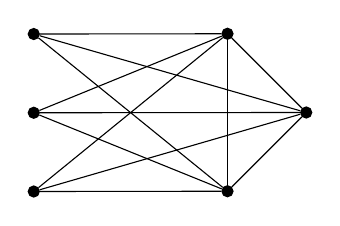
\begin{tikzpicture}[black/.style={circle,draw,fill=black,inner sep=0pt,minimum width=4pt}]
\def\n{3}
\def\m{3}
\def\ang{90}
\foreach \number in {1,...,\n}
{
	\mycount=\number
	\advance\mycount by -1
	\multiply\mycount by \ang
	\advance\mycount by 270
	\node[black,xshift=70,yshift=57] (k\number) at (\the\mycount:1cm) {};
}
\foreach \x in {1,...,\n}
	\foreach \y in {\x,...,\n}
		\draw (k\x) -- (k\y);

\foreach \number in {1,...,\m}
{
	\node[black] (\number) at (0,\number) {};
	\foreach \x in {1,...,\n}
		\draw (\number) -- (k\x);
}
\end{tikzpicture}
\newline
\newline
$K_2$:
\newline
\newline
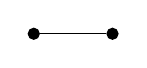
\begin{tikzpicture}[black/.style={circle,draw,fill=black,inner sep=0pt,minimum width=4pt}]
	\node[black] (a) at (0,0) {};
	\node[black] (b) at (1,0) {};
	\draw (a) -- (b);
\end{tikzpicture}
\newline
\newline
$P_4$:
\newline
\newline
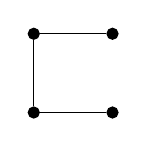
\begin{tikzpicture}[black/.style={circle,draw,fill=black,inner sep=0pt,minimum width=4pt}]
	\node[black] (a) at (0,0) {};
	\node[black] (b) at (0,1) {};
	\node[black] (c) at (1,0) {};
	\node[black] (d) at (1,1) {};
	\draw (a) -- (b);
	\draw (a) -- (c);
	\draw (b) -- (d);
\end{tikzpicture}
\newline
\newline
$K_{1,n}$:
\newline
\newline
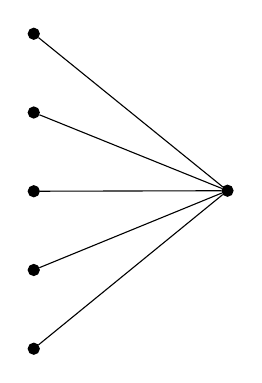
\begin{tikzpicture}[black/.style={circle,draw,fill=black,inner sep=0pt,minimum width=4pt}]
\def\n{1}
\def\m{5}
\def\ang{90}
\foreach \number in {1,...,\n}
{
	\mycount=\number
	\advance\mycount by -1
	\multiply\mycount by \ang
	\advance\mycount by 270
	\node[black,xshift=70,yshift=114] (k\number) at (\the\mycount:1cm) {};
}
\foreach \x in {1,...,\n}
	\foreach \y in {\x,...,\n}
		\draw (k\x) -- (k\y);

\foreach \number in {1,...,\m}
{
	\node[black] (\number) at (0,\number) {};
	\foreach \x in {1,...,\n}
		\draw (\number) -- (k\x);
}
\end{tikzpicture}


\subsection{Basic properties}
\begin{itemize}
	\item If $G$ is a split graph, then $\overline{G}$ is a split graph.
	\item If $G$ is a split graph with partition $(S,K)$, $S$ an independent set and $K$
		a clique, then exactly one of the following holds:
		\begin{enumerate}
			\item $|S|=\alpha(G)$ and $|K|=\omega(G)$.
			\item $|S|=\alpha(G)$ and $|K|=\omega(G)-1$, and there exists a vertex
				$x\in S$ such that $K+x$ is a complete graph.
			\item $|S|=\alpha(G)-1$ and $|K|=\omega(G)$, and there exists a vertex
				$y\in K$ such that $S+y$ is independent.
		\end{enumerate}
	\item $G$ is a split graph if and only if both $G$ and $\overline{G}$ are chordal.\cite{Golumbic}
\end{itemize}


\section{Characterizations}
\subsection{Vertex ordering}
Let $G$ be a graph with degree sequence $d_1\le\cdots\le d_n$, and let $m$ be
the largest $i$ with $d_i\ge i-1$. Then $G$ is a split graph if and only if
\[\sum_{i=1}^md_i=m(m-1)+\sum_{i=m+1}^nd_i.\]
Furthermore, if the above equality holds, then $\omega(G)=m$.\cite{Hammer}


\subsection{Forbidden subgraphs}
$G$ is a split graph if and only if $G$ contains no induced subgraph
isomorphic to any of $C_4$, $\overline{C_4}$, or $C_5$.\cite{Hammer}


\section{Optimization problems}
\subsection{Colouring}
Split graphs are in particular chordal graphs. \cite{Golumbic} gives an
algorithm to colour chordal graphs in linear time, so split graphs can also be
coloured in linear time. This is a very hard problem in general, and colouring
an arbitrary graph takes exponential time.


\subsection{Maximum clique}
$m$ as defined in the vertex ordering characterization of split graphs allows
us to find a maximum clique: the $m$ vertices of largest degree form a maximum
clique on $G$. This process can be done in linear time.


\subsection{Maximum independent set}
Let $K$ be the maximum clique obtained using the above method.
$V(G)\setminus K$ is an independent set, so we know from the basic properties
that exactly one of the three cases is possible, and $\alpha(G)$ is either
$|V(G)\setminus K|$ or $|V(G)\setminus K|+1$. If it is $|V(G)\setminus K|+1$,
then there exists a vertex $y\in K$ such that $V(G)\setminus K + y$ is still
independent. We can search $K$ for such a vertex in linear time, and we're
done.


\subsection{Minimum clique covering}
We know that $\overline{G}$ is a split graph, so we can colour $\overline{G}$
using the algorithm given in \cite{Golumbic} to get a set of colour classes,
all of which are independent sets in $\overline{G}$, hence cliques in $G$.
Since the colouring is optimal, the corresponding clique cover is minimal.


\bibliography{p5}
\bibliographystyle{plain}


\end{document}
